\newcommand{\paramI}[1]{\text{-}\ensuremath{#1}}
\newcommand{\param}[1]{\text{\--\--}\ensuremath{#1}}

\chapter{TRAVeLer - Template RnA VisuaLization}

Traveler je konzolova aplikacia programovana v C++ a je urceny pre operacne systemy UNIX-oveho typu.
Vyvyjany a testovany bol na Linux-e a FreeBSD. Podpora ostatnych systemov nieje zarucena.

\section{Instalacia}

Pozadovane programove vybavenie je:
\begin{itemize}
  \item gcc verzie aspon 4.9.2
\end{itemize}

Pri testovani boli zaznamenane problemy s regularnymi vyrazmi, ktore nam pomahaju pri nacitavani
vstupnych suborov. Problem bol pri verzii gcc 4.7.2, ktora plne nepodporovala potrebne vyrazy.

Traveler prelozime zo zdrojovych kodov postupnostou prikazov z korenoveho adresara:
\begin{itemize}
  \item cd src/
  \item make build
    \\
    Nasledne spustitelny subor je $src/build/traveler$.
\end{itemize}

\section{Argumenty programu}

Ak predpokladame, ze program lezi na $PATH$, spustame ho nasledovne:

\begin{code}[frame=none]
traveler [-h|--help]
traveler [OPTIONS] <TREES>

OPTIONS:
  [-a|--all [--overlaps] [--colored] <FILE_OUT>]
  [-t|--ted <FILE_MAPPING_OUT>]
  [-d|--draw [--overlaps] [--colored] <FILE_MAPPING_IN> <FILE_OUT>]
  [--debug]

TREES:
  <-mt|--match-tree> FILE_FASTA
  <-tt|--template-tree> [--type DOCUMENT_TYPE] DOCUMENT FILE_FASTA
\end{code}

Strucnu napovedu k programu dostaneme standardnym \paramI{h} alebo \param{help} argumentom.

Prepinacmi \param{ted} a \param{draw} vieme oddelit fazu pocitania vzdialenosti pomocou TEDu a nasledneho kreslenia.

Prepinac \param{overlaps} po nakresleni obrazku v nom vyznaci vsetky miesta prekryvov, ak nejake vznikli.
Zaroven ich pocet vypise do samostatneho suboru. Nasledne rychlejsie dokazeme identifikovat molekuly, ktore
potrebuju zvysenu pozornost.

Prepinac \param{colored} aktivuje farebne zvyraznovanie zmien v strukture stromu oproti sablone.
Pouzivame nasledovne kodovanie farbami:

\begin{tabular}{@{$\bullet$ }ll}
  $Cervena$ & vlozene bazy
  \\
  $Zelena$  & editovane bazy
  \\
  $Modra$   & bazy ktore sme potrebovali presunut
  \\
  $Hneda$   & podstromy prekreslenych multibranch loop
\end{tabular}
\\

Farbami zvyraznujeme zmeny v strome, to znamena, ze ak sa bazovy par zmeni v jednej baze,
cely bude oznaceny ako editovany.

Modrou oznacujeme casti, ktore sme z nejakeho dovodu potrebovali presunut a prekreslit. Typickym prikladom
je prekreslenie loopy po vlozeny/zmazani nejakej bazy. Vtedy sme vlozili napriklad 1 bazu ale potrebovali
presunut dalsich 10 ktore uz v loop boli.
% TODO priklad

Hnedou farbou oznacujeme cele podstromy multibranch loopy, ktoru sme museli prekreslit.
V tychto pripadoch vznikaju casto velke prekryvy a tymto ich odlisujeme od ostatnych, necakanych.

Prepínač \param{match-tree} nám určuje RNA molekulu ktorú ideme vizualizovať, \param{template-tree}
šablónu. Strom vizualizovanej molekuly sa načítava iba z fasta súboru, kdežto pri šablónovej molekule
potrebujeme aj jej obrázok. Viac informácii ohľadom parametra \param{type} nájdete v kapitole \nameref{kap:rozsirenie}.

\subsection{Format fasta suboru}

Ako format suborov kodujucich stromy pouzivame trochu upraveny fasta format.

Subor na prvom riadku obsahuje nazov molekuly hned za znakom $>$ az po prvu medzeru.
Na dalsich riadkoch obsahuje znaky sekvencie RNA a znaky kodujuce sekundarnu strukturu.
Je zvykom, ze riadky su siroke najviac 80 znakov.

Fasta subor pre sablonovu molekulu RNA potrebuje iba nazov a zatvorkovanie, pre
vizualizovanu molekulu aj sekvenciu. Je to dane tym, ze sekvenciu si vieme vybrat z obrazka sablony.

\section{Priklad vstupu}

Teraz uvedieme priklad vstupu pre malu podjednotku ribozomalnej RNA mysi, konkretne priklad
fasta suboru \ref{obr:mouse_fasta}, podporovaneho formatu post script suboru \ref{obr:mouse_ps_text}
a nasledne aj obrazok vizualizacie v post script subore \ref{obr:mouse_ps}.

\begin{pozn}
  Podporujeme iba jeden format PostScript súborov - ten používa databáza CRW publikovaná \citet{CRW}.
  Ďalšie rozšírenia podpory inych formatov rozoberáme v kapitole \nameref{kap:rozsirenie}.
\end{pozn}

\begin{figure}[H]
\begin{code}[fontsize=\scriptsize, frame=none, samepage=true]
>mouse
UACCUGGUUGAUCCUGCCAGUAGCAUAUGCUUGUCUCAAAGAUUAAGCCAUGCAUGUCUAAGUACGCACGGCCGGUACAG
UGAAACUGCGAAUGGCUCAUUAAAUCAGUUAUGGUUCCUUUGGUCGCUCGCUCCUCUCCUACUUGGAUAACUGUGGUAAU
UCUAGAGCUAAUACAUGCCGACGGGCGCUGACCCCCCUUCCCGGGGGGGGAUGCGUGCAUUUAUCAGAUCAAAACCAACC
CGGUGAGCUCCCUCCCGGCUCCGGCCGGGGGUCGGGCGCCGGCGGCUUGGUGACUCUAGAUAACCUCGGGCCGAUCGCAC
GCCCCCCGUGGCGGCGACGACCCAUUCGAACGUCUGCCCUAUCAACUUUCGAUGGUAGUCGCCGUGCCUACCAUGGUGAC
CACGGGUGACGGGGAAUCAGGGUUCGAUUCCGGAGAGGGAGCCUGAGAAACGGCUACCACAUCCAAGGAAGGCAGCAGGC
GCGCAAAUUACCCACUCCCGACCCGGGGAGGUAGUGACGAAAAAUAACAAUACAGGACUCUUUCGAGGCCCUGUAAUUGG
AAUGAGUCCACUUUAAAUCCUUUAACGAGGAUCCAUUGGAGGGCAAGUCUGGUGCCAGCAGCCGCGGUAAUUCCAGCUCC
AAUAGCGUAUAUUAAAGUUGCUGCAGUUAAAAAGCUCGUAGUUGGAUCUUGGGAGCGGGCGGGCGGUCCGCCGCGAGGCG
AGUCACCGCCCGUCCCCGCCCCUUGCCUCUCGGCGCCCCCUCGAUGCUCUUAGCUGAGUGUCCCGCGGGGCCCGAAGCGU
UUACUUUGAAAAAAUUAGAGUGUUCAAAGCAGGCCCGAGCCGCCUGGAUACCGCAGCUAGGAAUAAUGGAAUAGGACCGC
GGUUCUAUUUUGUUGGUUUUCGGAACUGAGGCCAUGAUUAAGAGGGACGGCCGGGGGCAUUCGUAUUGCGCCGCUAGAGG
UGAAAUUCUUGGACCGGCGCAAGACGGACCAGAGCGAAAGCAUUUGCCAAGAAUGUUUUCAUUAAUCAAGAACGAAAGUC
GGAGGUUCGAAGACGAUCAGAUACCGUCGUAGUUCCGACCAUAAACGAUGCCGACUGGCGAUGCGGCGGCGUUAUUCCCA
UGACCCGCCGGGCAGCUUCCGGGAAACCAAAGUCUUUGGGUUCCGGGGGGAGUAUGGUUGCAAAGCUGAAACUUAAAGGA
AUUGACGGAAGGGCACCACCAGGAGUGGGCCUGCGGCUUAAUUUGACUCAACACGGGAAACCUCACCCGGCCCGGACACG
GACAGGAUUGACAGAUUGAUAGCUCUUUCUCGAUUCCGUGGGUGGUGGUGCAUGGCCGUUCUUAGUUGGUGGAGCGAUUU
GUCUGGUUAAUUCCGAUAACGAACGAGACUCUGGCAUGCUAACUAGUUACGCGACCCCCGAGCGGUCGGCGUCCCCCAAC
UUCUUAGAGGGACAAGUGGCGUUCAGCCACCCGAGAUUGAGCAAUAACAGGUCUGUGAUGCCCUUAGAUGUCCGGGGCUG
CACGCGCGCUACACUGACUGGCUCAGCGUGUGCCUACCCUGCGCCGGCAGGCGCGGGUAACCCGUUGAACCCCAUUCGUG
AUGGGGAUCGGGGAUUGCAAUUAUUCCCCAUGAACGAGGAAUUCCCAGUAAGUGCGGGUCAUAAGCUUGCGUUGAUUAAG
UCCCUGCCCUUUGUACACACCGCCCGUCGCUACUACCGAUUGGAUGGUUUAGUGAGGCCCUCGGAUCGGCCCCGCCGGGG
UCGGCCCACGGCCCUGGCGGAGCGCUGAGAAGACGGUCGAACUUGACUAUCUAGAGGAAGUAAAAGUCGUAACAAGGUUU
CCGUAGGUGAACCUGCGGAAGGAUCAUUA
...(((((.......))))).((((((((((.(((((((((.....(((.(((..((...(((....((..........)
)...)))))......(((......((((..((..((....(((..................((((....(((((((....
.))))))).....)))).......((((...((((((......))))))...))))....((((((.......(((((.(
(((...((((.((((((((....))))))))..)))).))))....)))))......))))))...........((((.(
(((......))))))))....)))...))))..))))(((..(.(((....((((((((.......)))))))))))...
..))))...((((((((....))))...))))))).((((((..........)))))).((((....))))...))))))
.).....(.(((...(((((...))))).)))).)).))))))....(((((((((.(((....)))..)))))).))).
.....(((.(((.......)))).)).........((((((.......((((.....((....)).......))))))))
)).))))))))))..........(((.......((((...(((.......(((.(((((((((((((.((((....))))
....))))))))..)))))))).......((((.(((((...(((((((......)))))))....))))))))).....
................................................................................
...........................................(((((((((..(((((((((..((((((((...(((.
.....)))......))))))))..))....(..((....)))))))))).))))).))))...)))...))))....(((
(((...((...((((.........))))...))))))))..........((((((.(((..((((((((.(((((....)
))))))))))))..)))...((....))...)))....))).)))..(((.....((((....))))....)))......
..(((((.(((((((..((..((((((((((((((((....((((........))))........(((((((....((((
(........((((((........))))))......)))))...((.((((..(((((((((...(((((((((....)))
..((((......))))..)))))).....((((.(((.((((..((((....(((..((((....)))).)))....)))
)..)))))))..((((((((.....))))))))....))))...)))).)))...).))))))).....)))))))...)
).))))))).))...(((((((.....(((.......((..((((....))))..)).....))).....)))))))...
...(...((((((((........))))))))...).....))))).....((((((((.......))))))))......)
)...)))))))))).))....((.((.(.((((((((.((.((((((((((((..(((((((((((((((.(((((((((
(((.....))))))))))))...)))))))))))))))..))))))))))))).)))))))))..).))..))....(((
(((((((....))))))))))........
\end{code}
\caption{Priklad fasta suboru}
\label{obr:mouse_fasta}
\end{figure}

\begin{figure}[H]
\begin{code}[fontsize=\scriptsize, frame=none, samepage=true]
%!
/lwline {newpath moveto lineto stroke} def
  ...
434.00 -129.00 422.00 -138.00 lwline
0.00 setlinewidth
446.00 -421.00 446.00 -412.00 lwline
306.00 -283.00 306.00 -273.00 lwline
  ...
(U) 303.30 -273.00 lwstring
(A) 303.30 -265.00 lwstring
(C) 303.30 -257.00 lwstring
(C) 303.50 -248.68 lwstring
(U) 311.24 -246.68 lwstring
(G) 318.99 -244.68 lwstring
  ...
\end{code}
\caption{Priklad podporovaneho formatu post script suboru}
\label{obr:mouse_ps_text}
\end{figure}

\begin{figure}
  \makebox[\textwidth]{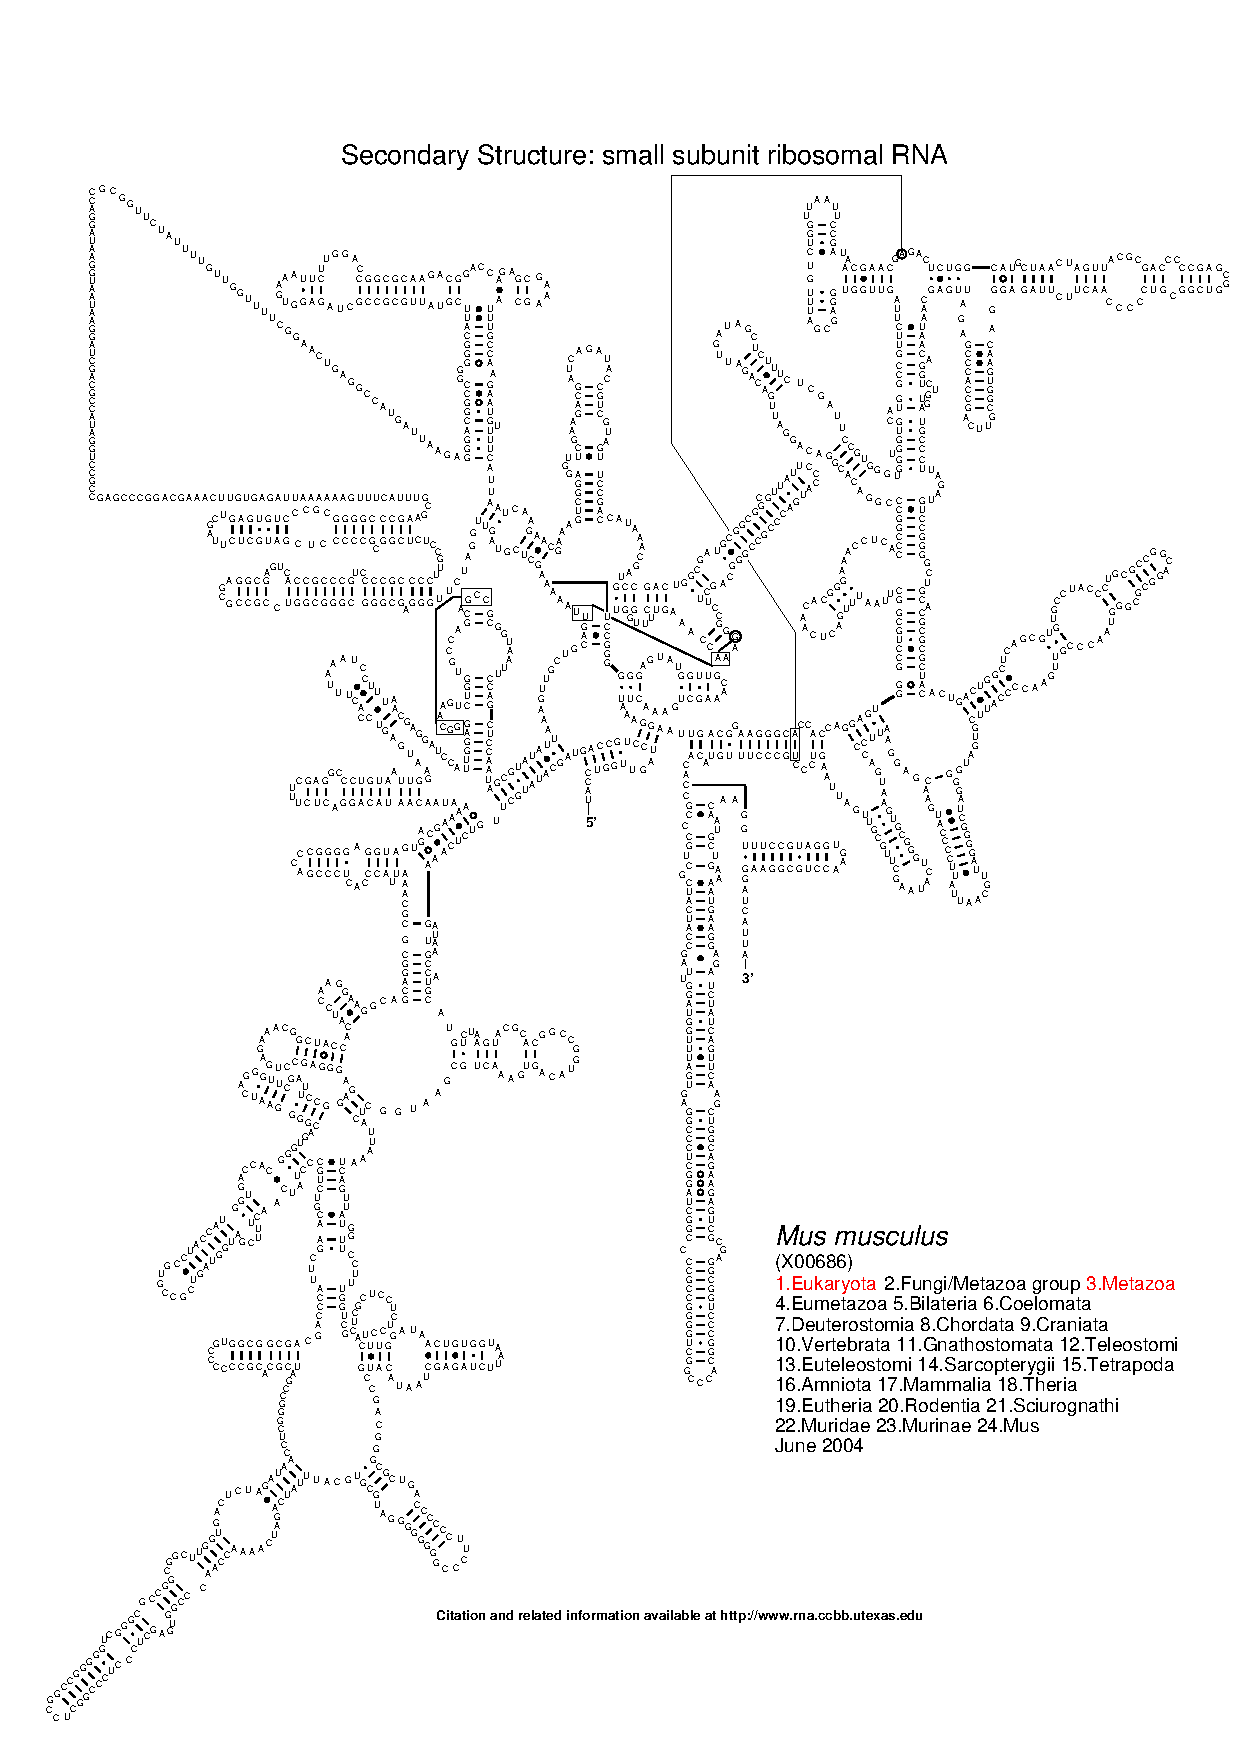
\includegraphics[width=\textwidth]{../img/mouse}}
  \caption{Priklad vstupneho obrazka}
  \label{obr:mouse_ps}
\end{figure}

\section{Vystupne subory}

Program generuje 2 druhy vystupov. Prvym je ulozenie tabulky mapovania TED algoritmu a druhym su obrazky
vo formate SVG a PS. \\

Oznacme $T1$ strom sablony a $T2$ vizualizovany strom.

Format mapovacieho suboru je nasledovny: \\
Prvy riadok obsahuje $DISTANCE: n$, kde $n$ je
editacna vzdialenost medzi $T1$ a $T2$.

Ostatne riadky su vo formate $i$ $j$, kde $i, j \ge 0$. Inymi slovami:
\begin{itemize}
  \item 1 2 - prvy vrchol z $T1$ potrebujeme namapovat na druhy vrchol z $T2$
  \item 0 2 - do vysledneho stromu vkladame druhy vrchol z $T2$
  \item 1 0 - zo stromu $T1$ mazeme prvy vrchol
\end{itemize}

PostScript subor je zlozeny z hlavicky v ktorej su definicie kresliacich funkcii za
ktorymi su riadky kreslenia molekuly. Priklad je na obrazku \ref{obr:ps_out}.

Najprv definujeme operacie kreslenia v hlavicke suboru - $lwline$, $lwstring$ a $lwarc$ - kreslenie ciar,
textu a kruznic. Za ktorymi nasleduje samotne kreslenie molekuly. \\

Podobne funguje kreslenie v SVG subore ktoreho priklad je na obrazku \ref{obr:svg_out}.
Elementy $<text>$ vypisuju na danu poziciu text, $<line>$
naopak kreslia ciary a $<circle>$ zase kruznice.

% TODO pouzivat cele priklady malej existujucej molekuly
\begin{figure}
\begin{code}[fontsize=\scriptsize, frame=none, samepage=true]
%!
/lwline {newpath moveto lineto stroke} def
/lwstring {moveto show} def
/lwarc {newpath gsave translate scale /rad exch def /ang1 exch def /ang2 exch def 0.0 0.0
  rad ang1 ang2 arc stroke grestore} def
/Helvetica findfont 8.00 scalefont setfont
0.36 0.46 scale
219.18 1384.80 translate
0              1              0               setrgbcolor
(5')            298.311        -268.09         lwstring
0              0              0               setrgbcolor
(U)             303.3          -273            lwstring
(A)             303.3          -265            lwstring
(C)             303.3          -257            lwstring
(C)             303.501        -248.682        lwstring
305.5          -241.809       302.5          -230.191        lwline
(U)             311.246        -246.682        lwstring
  ...
showpage
\end{code}
\caption{Format vystupneho PostScript suboru}
\label{obr:ps_out}
\end{figure}

\begin{figure}
\begin{code}[fontsize=\scriptsize, frame=none, samepage=true]
<svg
  xmlns="http://www.w3.org/2000/svg"
  xmlns:xlink="http://www.w3.org/1999/xlink"
  width="1133.333333"
  height="1466.666667"
  viewBox="0 0 1139.172822px 1450.347571px"
  style="
    font-size: 8px; 
    stroke: none; 
    font-family: Helvetica; ">

  <text 
    x="517.486977"
    y="603.524781"
    style="
      stroke: rgb(0, 255, 0); ">5'</text>

  <line 
    x1="681.175823"
    y1="650.435118" 
    x2="681.175823"
    y2="662.435118"
    style="
      stroke: rgb(0, 0, 0); 
      stroke-width: 2; "/>


  <circle 
    cx="616.350806"
    cy="427.616196"
    r="6.276645"
    style="
      stroke: rgb(0, 0, 0); 
      fill: none; "/>

  ...
</svg>
\end{code}
\caption{Format vystupneho SVG suboru}
\label{obr:svg_out}
\end{figure}


\section{Rozšírenie podpory iných vstupných obrázkov}
\label{kap:rozsirenie}

Ako sme už uviedli, momentálne podporujeme iba jediny vstupny format vstupných obrázkov.
Je ním PostScript formát používaný databázou CRW od autorov \citet{CRW}.

\begin{definice}
  Extractor bude nejaky objekt ktory vie zo suboru urciteho typu vynat potrebne
  polozky reprezentujuce RNA sekvenciu a poziciu baz na obrazku.
\end{definice}

Pri tvorbe aplikácie sme už mysleli na budúcnosť a načítavanie súboru robíme v jednom lahko
rozsiritelnom module. Ten sa na zaklade typu v parametre \param{template-tree} rozhoduje
aky extractor pouzit. Predvoleny a jediny implementovany je PostScript extractor fungujuci
nad subormi z CRW databazy.

Na implementovanie extractora potrebujeme implementovat existujuce rozhranie $extractor$,
co znamena implementovat metodu $init$ s parametrom nazvu suboru.

Jej uloha je zo suboru ziskat sekvenciu RNA a pozicie baz.

Poslednou ulohou je pridat dvojicu $(názov\_exctractora, extractor)$ do tabulky implementovanych
v metode $create\_exctractors()$.

Naslednym volanim \param{template-tree} \param{type} $nazov\_extractora$ zacneme
pouzivat nas novo implementovany extractor.


